\chapter{User Interface}

\section{Main Window}
In the Main Window you can see the following editors and views:
\begin{itemize}
	\item Architecture Editor
	\item Role View
	\item Workflow/Task View
	\item Minimap
\end{itemize}

\begin{figure}[h!]
\begin{center}
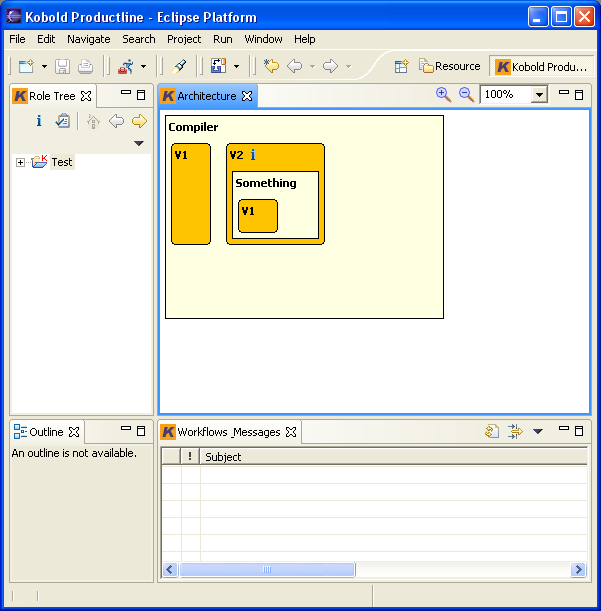
\includegraphics[width=10cm]{main.png}
   \caption{Main Window}
\label{wizard3}
\end{center}
\end{figure}\par

The menu offers you in addition to the Eclipse standard options the following
possibilities:
\begin{itemize}
	\item Checking out a product
	\item Exporting through GXL
\end{itemize}
Look up the explanations in the "Tutorial" section.

\section{Architecture Editor}

The Architecture Editor displays the architecture of the product,
or product line respectively, that is selected in the Role View. \par

Architectures are directed graphs that consist of nodes and edges. 
Nodes represent components, variants and files. Directed edges represent
any relationship between nodes.\par

The Architecture Editor offers you the following options:
\begin{itemize}
	\item Creating a Core Asset
	\item Creating a variant
	\item Creating a component
	\item Creating a version
	\item Creating a meta node
	\item Deleting a core asset, component, variant or version
	\item Deleting a meta node
	\item Creating a dependency edge
	\item Creating an exclusion edge
	\item Deleting an edge
	\item Marking a component as "deprecated"
	\item Moving an item
	\item Changing the size of an item
	\item Filtering the Architecture View
	\item Creating a custom component
	\item Deleting a custom component
\end{itemize}
Look up the explanations in the "Tutorial" section.

\section{Role View}

The Role View shows the current projects that are checked out in your workspace 
(see \ref{roletree}).
A project can either be a product or a product line. You can navigate between the 
different projects by selecting them. The open tree in the Role View displays the
role of the current user in the project. You can also see the architecture and its 
elements.

\begin{figure}[h!]
\begin{center}

\includegraphics[width=10cm]{roletree.png}
   \caption{Role View}
\label{roletree}
\end{center}
\end{figure}\par

When you right-click on a project, a context menu will open where you can choose 
between different actions (see \ref{rolekontext}). Among those are:

\begin{itemize}
	\item Creating a product
	\item Renaming a product
	\item Changing a product
	\item Setting a product on deprecated
	\item Setting a module on deprecated
	\item Creating a user
	\item Changing a user role
\end{itemize}
Look up the explanations in the "Tutorial" section.

\begin{figure}[h!]
\begin{center}

\includegraphics[width=10cm]{rolekontext.png}
   \caption{Project Context Menu}
\label{rolekontext}
\end{center}
\end{figure}\par



\section{Workflow/Task View}

In the bottom of the window you can see the Workflow/Task View which displays all 
the messages and workflows for the current user (see \ref{workflow}). 

\begin{figure}[h!]
\begin{center}

\includegraphics[width=15cm]{workflow.png}
   \caption{Workflow/Task View}
\label{workflow}
\end{center}
\end{figure}\par

Double-click on an entry and a 
separate dialog will be opened where you can read the details of that message or
workflow (see \ref{workflowdialog}).

\begin{figure}[h!]
\begin{center}

\includegraphics[width=5cm]{workflowdialog.png}
   \caption{Message Dialog}
\label{workflowdialog}
\end{center}
\end{figure}\par

When you right-click on a message, a context menu will open where you can choose 
between the different actions (see \ref{workflowkontext}). Among these are:

\begin{itemize}
	\item Fetching messages
	%\item Deleting the selected message
	\item Filtering sent messages
\end{itemize}
Look up the explanations in the "Tutorial" section.

\begin{figure}[h!]
\begin{center}

\includegraphics[width=10cm]{workflowkontext.png}
   \caption{Message Context Menu}
\label{workflowkontext}
\end{center}
\end{figure}\par

The Architecture Editor offers you the following additional options:
\begin{itemize}
	\item Writing a mail
	\item Answering a mail
	\item Suggesting a file for a Core Group
	\item Dealing with a Core Group suggestion
\end{itemize}
Look up the explanations in the "Tutorial" section.

\section{Minimap}

The Minimap is on the left side beneath the Role View. It shows the whole architecture.
By clicking at one spot on the map, the Architecture Editor automatically centers on that
spot. 


\section{Server Administration Tool}

The Server Administration Tool provides you with an interface to your server. \par
To start the Server Administration Tool within Eclipse just select 'Run...' in the
'Run' menu from Eclipse and select the class
{\it ServerAdministrationTool}.
During the starting process you have to enter the URL and password of the server 
you want to administrate. Once the tool is started, you have the following 
possibilities:

\begin{itemize}
	\item create a product line
	\item delete a product line
	\item upgrade an existing user to PLE status
	\item remove PLE rights
	\item get a list of all existing commands
	\item exit the tool
\end{itemize}

\subsection{Creating a product line}
Enter the command "createpl". You are asked to enter the name of the new product
line. Once you confirmed your entry, the product line is created.

\subsection{Deleting a product line}
Enter the command "removepl". You are then asked to enter the name of the product
line you want to remove. Once you confirmed your entry, the product line is deleted.

\subsection{Upgrading an existing user to PLE status}
Enter the command "addple". You are asked to enter the name of the person you want
to upgrade as PLE. Finally, enter the name of the product line you want to assign
the new PLE to. Once you confirmed your entry, the user has PLE rights.

\subsection{Removing PLE rights}
Enter the command "removeple". You are asked to enter the name of the user who shall 
no longer have PLE rights. Also, enter the name of the product line you want to
remove the PLE from. Once you confirmed your entry, the user is no longer PLE of
the entered product line.

\subsection{Getting a list of all existing commands}
Enter the command "help" and you get a list of all the commands of this tool and
their meanings.

\subsection{Exiting the tool}
Enter the command "exit".